% $Id$
\section{The Diffusion Problem}
\label{DIFFUSION CHAP}

\begin{figure}
\centerline{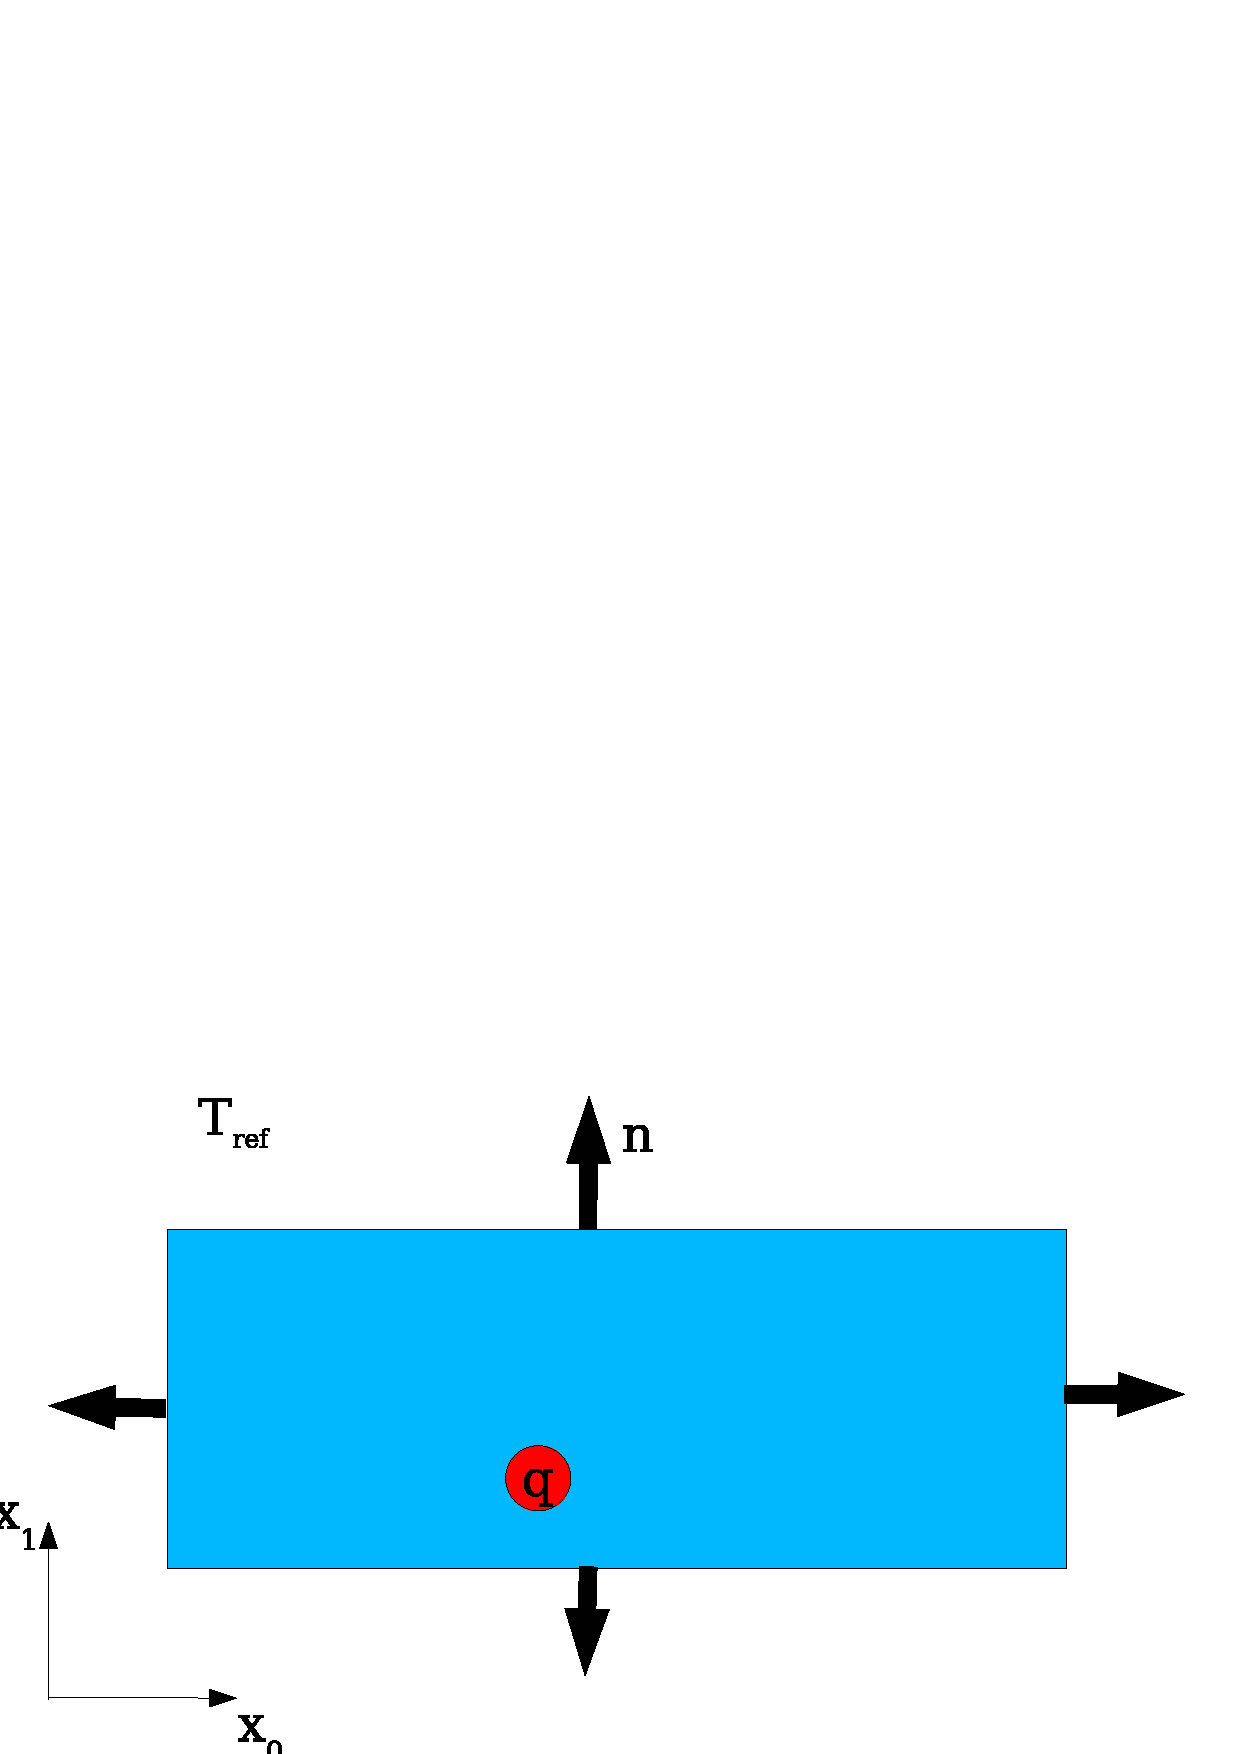
\includegraphics[width=\figwidth]{DiffusionDomain}}
\caption{Temperature Diffusion Problem with Circular Heat Source}
\label{DIFFUSION FIG 1}
\end{figure}

\subsection{\label{DIFFUSION OUT SEC}Outline}
In this chapter we will discuss how to solve the time dependent-temperature diffusion\index{diffusion equation} for
a block of material. Within the block there is a heat source which drives the temperature diffusion.
On the surface, energy can radiate into the surrounding environment.
\fig{DIFFUSION FIG 1} shows the configuration.

In the next \Sec{DIFFUSION TEMP SEC} we will present the relevant model. A 
time integration scheme is introduced to calculate the temperature at given time nodes $t^{(n)}$. 
We will see that at each time step a Helmholtz equation \index{Helmholtz equation} 
must be solved. 
The implementation of a Helmholtz equation solver will be discussed in \Sec{DIFFUSION HELM SEC}. 
In Section~\ref{DIFFUSION TRANS SEC} the solver of the Helmholtz equation is used to build a
solver for the temperature diffusion problem. 

\subsection{\label{DIFFUSION TEMP SEC}Temperature Diffusion}

The unknown temperature $T$ is a function of its location in the domain and time $t>0$. The governing equation
in the interior of the domain is given by
\begin{equation}
\rho c\hackscore p T\hackscore{,t} - (\kappa T\hackscore{,i})\hackscore{,i} = q
\label{DIFFUSION TEMP EQ 1}
\end{equation}
where $\rho c\hackscore p$ and $\kappa$ are given material constants. In case of a composite
material the parameters depend on their location in the domain. $q$ is
a heat source (or sink) within the domain. We are using Einstein summation convention \index{summation convention} 
as introduced in \Chap{FirstSteps}. In our case we assume $q$ to be equal to a constant heat production rate 
$q^{c}$ on a circle or sphere with center $x^c$ and radius $r$ and $0$ elsewhere:
\begin{equation}
q(x,t)=
\left\{ 
\begin{array}{lcl}
q^c  & & \|x-x^c\| \le r \\
     & \mbox{if} \\
0    &  & \mbox{else} \\
\end{array}
\right.
\label{DIFFUSION TEMP EQ 1b}
\end{equation}
for all $x$ in the domain and all time  $t>0$.

On the surface of the domain we are 
specifying a radiation condition 
which precribes the normal component of the flux $\kappa T\hackscore{,i}$ to be proportional
to the difference of the current temperature to the surrounding temperature $T\hackscore{ref}$:    
\begin{equation}
 \kappa T\hackscore{,i} n\hackscore i = \eta (T\hackscore{ref}-T) 
\label{DIFFUSION TEMP EQ 2}
\end{equation}
$\eta$ is a given material coefficient depending on the material of the block and the surrounding medium. 
As usual $n\hackscore i$ is the $i$-th component of the outer normal field \index{outer normal field}
at the surface of the domain. 

To solve the time dependent \eqn{DIFFUSION TEMP EQ 1} the initial temperature at time 
$t=0$ has to be given. Here we assume that the initial temperature is the surrounding temperature:
\begin{equation}
T(x,0)=T\hackscore{ref} 
\label{DIFFUSION TEMP EQ 4}
\end{equation}
for all $x$ in the domain. It is pointed out that 
the initial conditions satisfy the 
boundary condition defined by \eqn{DIFFUSION TEMP EQ 2}. 

The temperature is calculated at discrete time nodes $t^{(n)}$ where 
$t^{(0)}=0$ and  $t^{(n)}=t^{(n-1)}+h$ where $h>0$ is the step size which is assumed to be constant. 
In the following the upper index ${(n)}$ refers to a value at time $t^{(n)}$. The simplest
and most robust scheme to approximate the time derivative of the the temperature is 
the backward Euler
\index{backward Euler} scheme, see~\cite{XXX} for alternatives. The backward Euler 
scheme is based
on the Taylor expansion of $T$ at time $t^{(n)}$:
\begin{equation}
T^{(n-1)}\approx T^{(n)}+T\hackscore{,t}^{(n)}(t^{(n-1)}-t^{(n)})
=T^{(n-1)} - h \cdot T\hackscore{,t}^{(n)}
\label{DIFFUSION TEMP EQ 6}
\end{equation}
This is inserted into \eqn{DIFFUSION TEMP EQ 1}. By separating the terms at 
$t^{(n)}$ and  $t^{(n-1)}$ one gets for $n=1,2,3\ldots$
\begin{equation}
\frac{\rho c\hackscore p}{h} T^{(n)} - (\kappa T^{(n)}\hackscore{,i})\hackscore{,i} = q +  \frac{\rho c\hackscore p}{h} T^{(n-1)}
\label{DIFFUSION TEMP EQ 7}
\end{equation}
where $T^{(0)}=T\hackscore{ref}$ is taken form the initial condition given by \eqn{DIFFUSION TEMP EQ 4}.
Together with the natural boundary condition 
\begin{equation}
 \kappa T\hackscore{,i}^{(n)} n\hackscore i = \eta (T\hackscore{ref}-T^{(n)}) 
\label{DIFFUSION TEMP EQ 2222}
\end{equation}
taken from \eqn{DIFFUSION TEMP EQ 2}
this forms a boundary value problem that has to be solved for each time step. 
As a first step to implement a solver for the temperature diffusion problem we will 
first implement a solver for the  boundary value problem that has to be solved at each time step.

\subsection{\label{DIFFUSION HELM SEC}Helmholtz Problem}
The partial differential equation to be solved for $T^{(n)}$ has the form 
\begin{equation}
\omega u  - (\kappa u\hackscore{,i})\hackscore{,i} = f
\label{DIFFUSION HELM EQ 1}
\end{equation}
where $u$ plays the role of $T^{(n)}$ and we set
\begin{equation}
\omega=\frac{\rho c\hackscore p}{h} \mbox{ and } f=q+\frac{\rho c\hackscore p}{h}T^{(n-1)} \;.
\label{DIFFUSION HELM EQ 1b}
\end{equation}
With $g=\eta T\hackscore{ref}$ the radiation condition defined by \eqn{DIFFUSION TEMP EQ 2222}
takes the form 
\begin{equation}
\kappa u\hackscore{,i} n\hackscore{i} =  g - \eta u\mbox{ on } \Gamma
\label{DIFFUSION HELM EQ 2}
\end{equation}
The partial differential 
\eqn{DIFFUSION HELM EQ 1} together with boundary conditions of \eqn{DIFFUSION HELM EQ 2}
is called the Helmholtz equation \index{Helmholtz equation}. 

We want to use the \LinearPDE class provided by \escript to define and solve a general linear PDE such as the 
Helmholtz equation. We have used a special case of the \LinearPDE class, namely the
\Poisson class already in \Chap{FirstSteps}. 
Here we will write our own specialized sub-class of the \LinearPDE to define the Helmholtz equation
and use the \method{getSolution} method of parent class to actually solve the problem.

The form of a single PDE that can be handled by the \LinearPDE class is 
\begin{equation}\label{EQU.FEM.1}
-(A\hackscore{jl} u\hackscore{,l})\hackscore{,j}+D u =Y \; .
\end{equation}
We show here the terms which are relevant for the Helmholtz problem. 
The general form and systems is discussed in \Sec{SEC LinearPDE}.  
$A$, $D$ and $Y$ are the known coeffecients of the PDE. \index{partial differential equation!coefficients} 
Notice that $A$ is a matrix or tensor of order 2 and $D$ and $Y$ are scalar. 
They may be constant or may depend on their 
location in the domain but must not depend on the unknown solution $u$. 
The following natural boundary conditions \index{boundary condition!natural} that
are used in the \LinearPDE class have the form
\begin{equation}\label{EQU.FEM.2}
n\hackscore{j}A\hackscore{jl} u\hackscore{,l}+du=y  \;.
\end{equation}
where, as usual, $n$ denotes the outer normal field on the surface of the domain. Notice that 
the coefficient $A$ is already used in the PDE in \eqn{EQU.FEM.1}. $d$ and $y$ are given scalar coefficients.

By inspecting the Helmholtz equation \index{Helmholtz equation} 
we can easily assign values to the coefficients in the 
general PDE of the \LinearPDE class:
\begin{equation}\label{DIFFUSION HELM EQ 3}
\begin{array}{llllll}
A\hackscore{ij}=\kappa \delta\hackscore{ij} & D=\omega & Y=f \\
d=\eta & y= g &  \\
\end{array}
\end{equation}
$\delta\hackscore{ij}$ is the Kronecker symbol \index{Kronecker symbol} defined by $\delta\hackscore{ij}=1$ for
$i=j$ and $0$ otherwise.

We want to implement a 
new class which we will call \class{Helmholtz} that provides the same methods as the \LinearPDE class but
is described using the coefficients $\kappa$, $\omega$, $f$, $\eta$, 
$g$ rather than the general form given by \eqn{EQU.FEM.1}. 
Python's mechanism of subclasses allows us to do this in a very simple way.
The \Poisson class of the \linearPDEs module,
which we have already used in \Chap{FirstSteps}, is in fact a subclass of the more general
\LinearPDE class. That means that all methods (such as the \method{getSolution})
from the parent class \LinearPDE are available for any \Poisson object. However, new
methods can be added and methods of the parent class can be redefined. In fact,
the \Poisson class redefines the \method{setValue} of the \LinearPDE class which is called to assign 
values to the coefficients of the PDE. This is exactly what we will do when we define 
our new \class{Helmholtz} class:
\begin{python}
from esys.linearPDEs import LinearPDE
import numarray
class Helmholtz(LinearPDE):
   def setValue(self,kappa=0,omega=1,f=0,eta=0,g=0)
        ndim=self.getDim()
        kronecker=numarray.identity(ndim)
        self._LinearPDE_setValue(A=kappa*kronecker,D=omega,Y=f,d=eta,y=g)
\end{python}
\code{class Helmholtz(linearPDE)} declares the new \class{Helmholtz} class as a subclass 
of \LinearPDE which we have imported in the first line of the script. 
We add the method \method{setValue} to the class which overwrites the 
\method{setValue} method of the \LinearPDE class. The new method which has the 
parameters of the Helmholtz \eqn{DIFFUSION HELM EQ 1} as arguments 
maps the parameters of the coefficients of the general PDE defined 
in \eqn{EQU.FEM.1}. We are actually using the \method{_LinearPDE__setValue} of 
the \LinearPDE class. 
The coefficient \var{A} involves the Kronecker symbol. We use the
\numarray function \function{identity} which returns a square matrix with ones on the
main diagonal and zeros off the main diagonal. The argument of \function{identity} gives the order of the matrix.
The \method{getDim} of the \LinearPDE class object \var{self} to get the spatial dimensions of the domain of the
PDE. As we will make use of the \class{Helmholtz} class several times, it is convenient to 
put its definition into a file which we name \file{mytools.py} available in the \ExampleDirectory.
You can use your favourite editor to create and edit the file.   

An object of the \class{Helmholtz} class is created through the statments:
\begin{python}
from mytools import Helmholtz
mypde = Helmholtz(mydomain)
mypde.setValue(kappa=10.,omega=0.1,f=12)
u = mypde.getSolution()
\end{python}
In the first statement we import all definition from the \file{mytools.py} \index{scripts!\file{mytools.py}}. Make sure
that \file{mytools.py} is in the directory from where you started Python.
\var{mydomain} is the \Domain of the PDE which we have undefined here. In the third statment values are
assigned to the PDE parameters. As no values for arguments \var{eta} and \var{g} are
specified, the default values $0$ are used. \footnote{It would be better to use the default value 
\var{escript.Data()} rather then $0$ as then the coefficient would be defined as being not present and
would not be processed when the PDE is evaluated}. In the fourth statement the solution of the
PDE is returned. 

To test our \class{Helmholtz} class on a rectangular domain
of length $l\hackscore{0}=5$ and height $l\hackscore{1}=1$, we choose a simple test solution. Actually, we 
we take $u=x\hackscore{0}$ and then calculate the right hand side terms $f$ and $g$ such that
the test solution becomes the solution of the problem. If we assume $\kappa$ as being constant, 
an easy calculation shows that we have to choose $f=\omega \cdot x\hackscore{0}$. On the boundary we get
$\kappa n\hackscore{i} u\hackscore{,i}=\kappa n\hackscore{0}$.  
So we have to set $g=\kappa n\hackscore{0}+\eta x\hackscore{0}$. The following script \file{helmholtztest.py} 
\index{scripts!\file{helmholtztest.py}} which is available in the \ExampleDirectory
implements this test problem using the \finley PDE solver:
\begin{python}
from mytools import Helmholtz
from esys.escript import Lsup
from esys.finley import Rectangle
#... set some parameters ...
kappa=1.
omega=0.1
eta=10.
#... generate domain ...
mydomain = Rectangle(l0=5.,l1=1.,n0=50, n1=10)
#... open PDE and set coefficients ...
mypde=Helmholtz(mydomain)
n=mydomain.getNormal()
x=mydomain.getX()
mypde.setValue(kappa,omega,omega*x[0],eta,kappa*n[0]+eta*x[0])
#... calculate error of the PDE solution ...
u=mypde.getSolution()
print "error is ",Lsup(u-x[0])
\end{python}
The script is similar to the script \file{mypoisson.py} dicussed in \Chap{FirstSteps}.
\code{mydomain.getNormal()} returns the outer normal field on the surface of the domain. The function \function{Lsup}
is imported by the \code{from esys.escript import Lsup} statement and returns the maximum absulute value of its argument. 
The error shown by the print statement should be in the order of $10^{-7}$. As piecewise bi-linear interpolation is
used to approximate the solution and our solution is a linear function of the spatial coordinates one might 
expect that the error would be zero or in the order of machine precision (typically $\approx 10^{-15}$). 
However most PDE packages use an iterative solver which is terminated
when a given tolerance has been reached. The default tolerance is $10^{-8}$. This value can be altered by using the 
\method{setTolerance} of the \LinearPDE class. 

\subsection{The Transition Problem}
\label{DIFFUSION TRANS SEC}
Now we are ready to solve the original time dependent problem. The main 
part of the script is the loop over time $t$ which takes the following form:
\begin{python}
t=0
T=Tref
mypde=Helmholtz(mydomain)
while t<t_end:
      mypde.setValue(kappa,rhocp/h,q+rhocp/h*T,eta,eta*Tref)
      T=mypde.getSolution()
      t+=h
\end{python}
\var{kappa}, \var{rhocp}, \var{eta} and \var{Tref} are input parameters of the model. \var{q} is the heat source
in the domain and \var{h} is the time step size. Notice that the \class{Hemholtz} class object \var{mypde}
is created before the loop over time is entered while in each time step only the coefficients
are reset in each time step. This way some information about the representation of the PDE can be reused 
\footnote{The efficience can be improved further by setting the coefficients in the operator
\var{kappa}, \var{omega} and \var{eta} before entering the \code{while}-loop and only updating the coefficients
in the right hand side \var{f} and \var{g}. This needs a more careful implementation of the \method{setValue}
method but gives the advantage that the \LinearPDE class can save rebuilding the PDE operator.}. The variable \var{T}
holds the current temperature. It is used to calculate the right hand side coefficient \var{f} in the
Helmholtz equation in \eqn{DIFFUSION HELM EQ 1}. The statement \code{T=mypde.getSolution()} overwrites \var{T} with the 
temperature of the new time step $\var{t}+\var{h}$. To get this iterative process going we need to specify the
initial temperature distribution, which equal to $T\hackscore{ref}$.

The heat source \var{q} which is defined in \eqn{DIFFUSION TEMP EQ 1b} is \var{qc}
in an area defined as a circle of radius \var{r} and center \var{xc} and zero outside this circle.
\var{q0} is a fixed constant. The following script defines \var{q} as desired:  
\begin{python}
from esys.escript import length
xc=[0.02,0.002]
r=0.001
x=mydomain.getX()
q=q0*(length(x-xc)-r).whereNegative()
\end{python}
\var{x} is a \Data class object of
the \escript module defining locations in the \Domain \var{mydomain}.
The \function{length()} imported from the \escript module returns the 
Euclidean norm:
\begin{equation}\label{DIFFUSION HELM EQ 3aba}
\|y\|=\sqrt{
y\hackscore{i}
y\hackscore{i}
} = \function{esys.escript.length}(y)
\end{equation}
So \code{length(x-xc)} calculates the distances  
of the location \var{x} to the center of the circle \var{xc} where the heat source is acting.
Note that the coordinates of \var{xc} are defined as a list of floating point numbers. It is independently
converted into a \Data class object before being subtracted from \var{x}. The method \method{whereNegative} of
a \Data class object, in this case the result of the expression 
\code{length(x-xc)-r}, returns a \Data class which is equal to one where the object is negative and
zero elsewhere. After multiplication with \var{qc} we get a function with the desired property.

Now we can put the components together to create the script \file{diffusion.py} which is available in the \ExampleDirectory:
\index{scripts!\file{diffusion.py}}:
\begin{python}
from mytools import Helmholtz
from esys.escript import Lsup
from esys.finley import Rectangle
#... set some parameters ...
xc=[0.02,0.002]
r=0.001
qc=50.e6
Tref=0.
rhocp=2.6e6
eta=75.
kappa=240.
tend=5.
# ... time, time step size and counter ...
t=0
h=0.1
i=0
#... generate domain ...
mydomain = Rectangle(l0=0.05,l1=0.01,n0=250, n1=50)
#... open PDE ...
mypde=Helmholtz(mydomain)
# ... set heat source: ....
x=mydomain.getX()
q=qc*(length(x-xc)-r).whereNegative()
# ... set initial temperature ....
T=Tref
# ... start iteration:
while t<tend:
      i+=1
      t+=h
      print "time step :",t
      mypde.setValue(kappa=kappa,omega=rhocp/h,f=q+rhocp/h*T,eta=eta,g=eta*Tref)
      T=mypde.getSolution()
      T.saveDX("T%d.dx"%i)
\end{python}
The script will create the files \file{T.1.dx},
 \file{T.2.dx}, $\ldots$, \file{T.50.dx} in the directory where the script has been started. The files give the 
temperature distributions at time steps $1$, $2$, $\ldots$, $50$ in the \OpenDX file format. 

\begin{figure}
\centerline{
\includegraphics[width=\figwidth]{DiffusionRes1}}
\centerline{
\includegraphics[width=\figwidth]{DiffusionRes16}}
\centerline{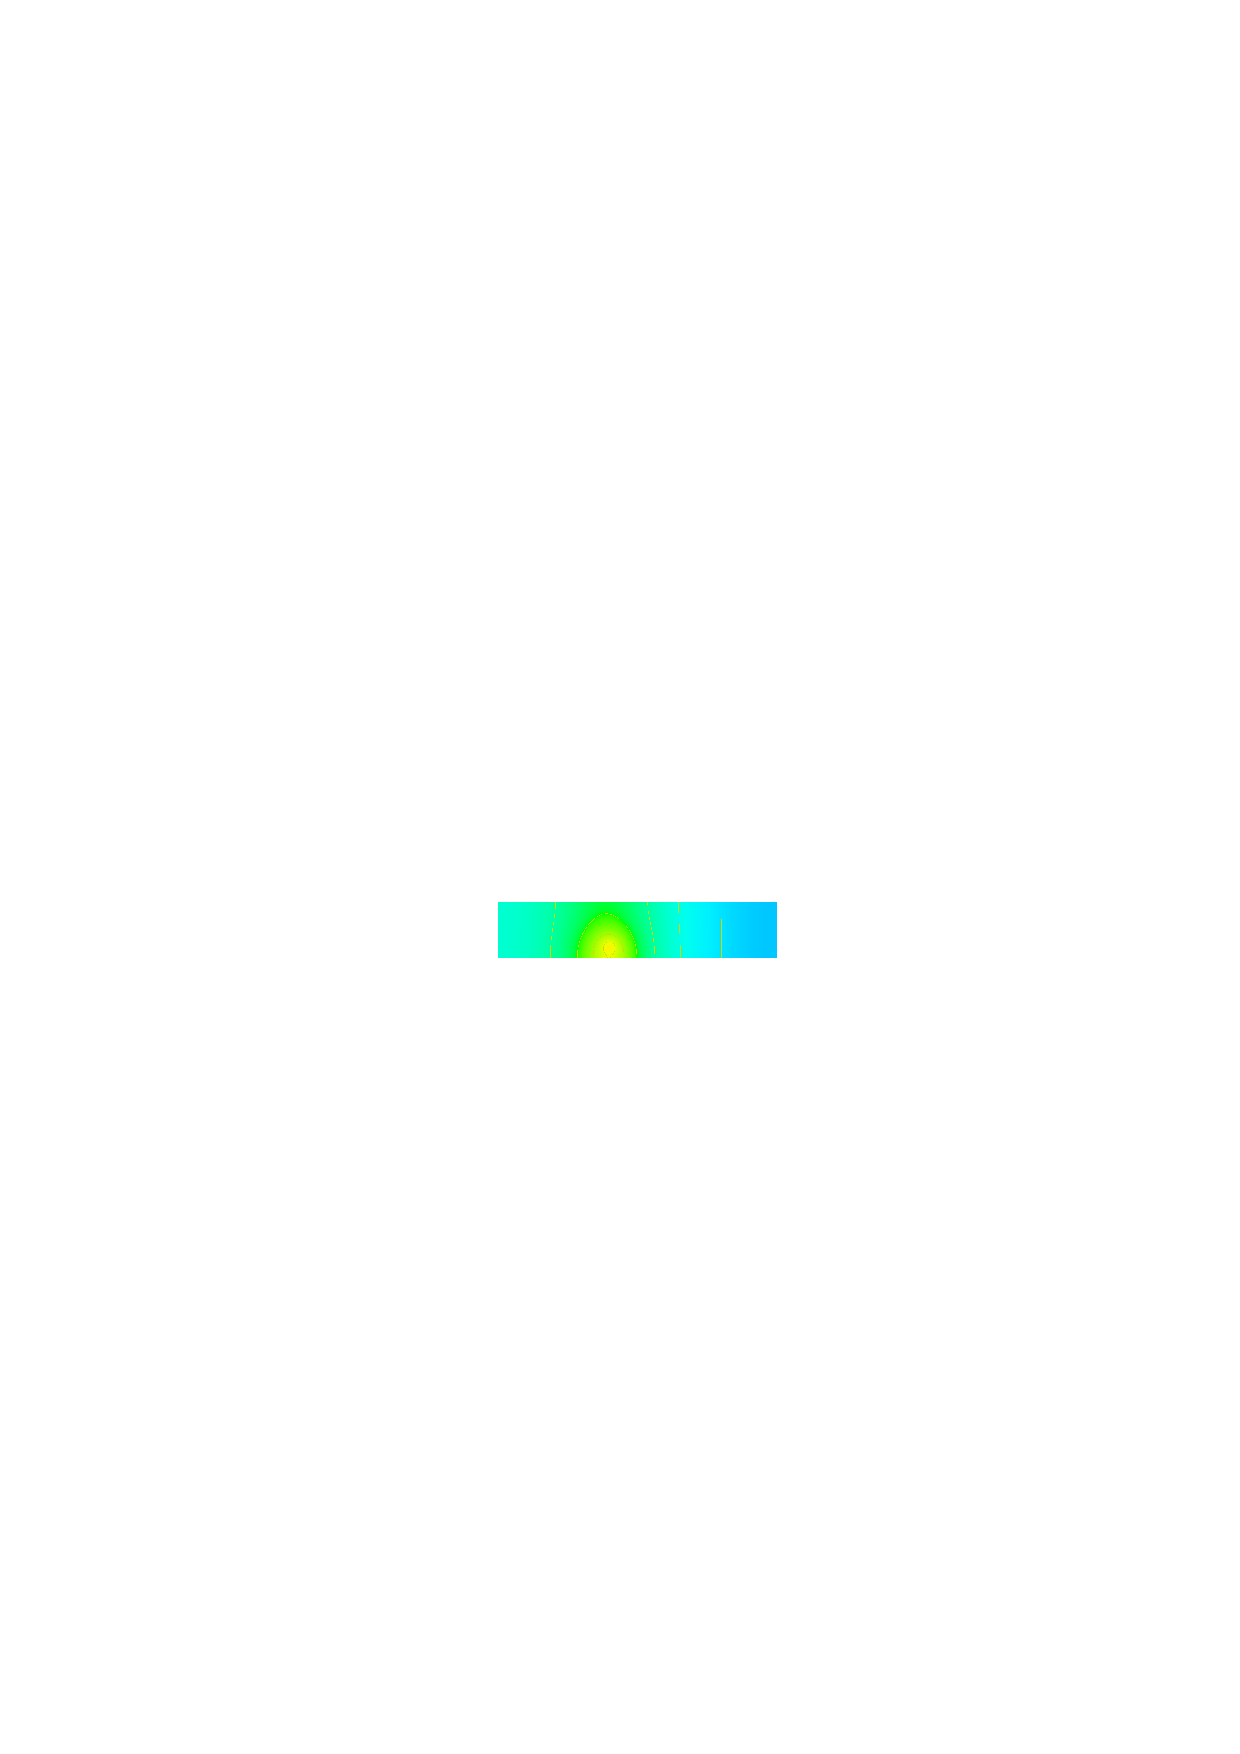
\includegraphics[width=\figwidth]{DiffusionRes32}}
\centerline{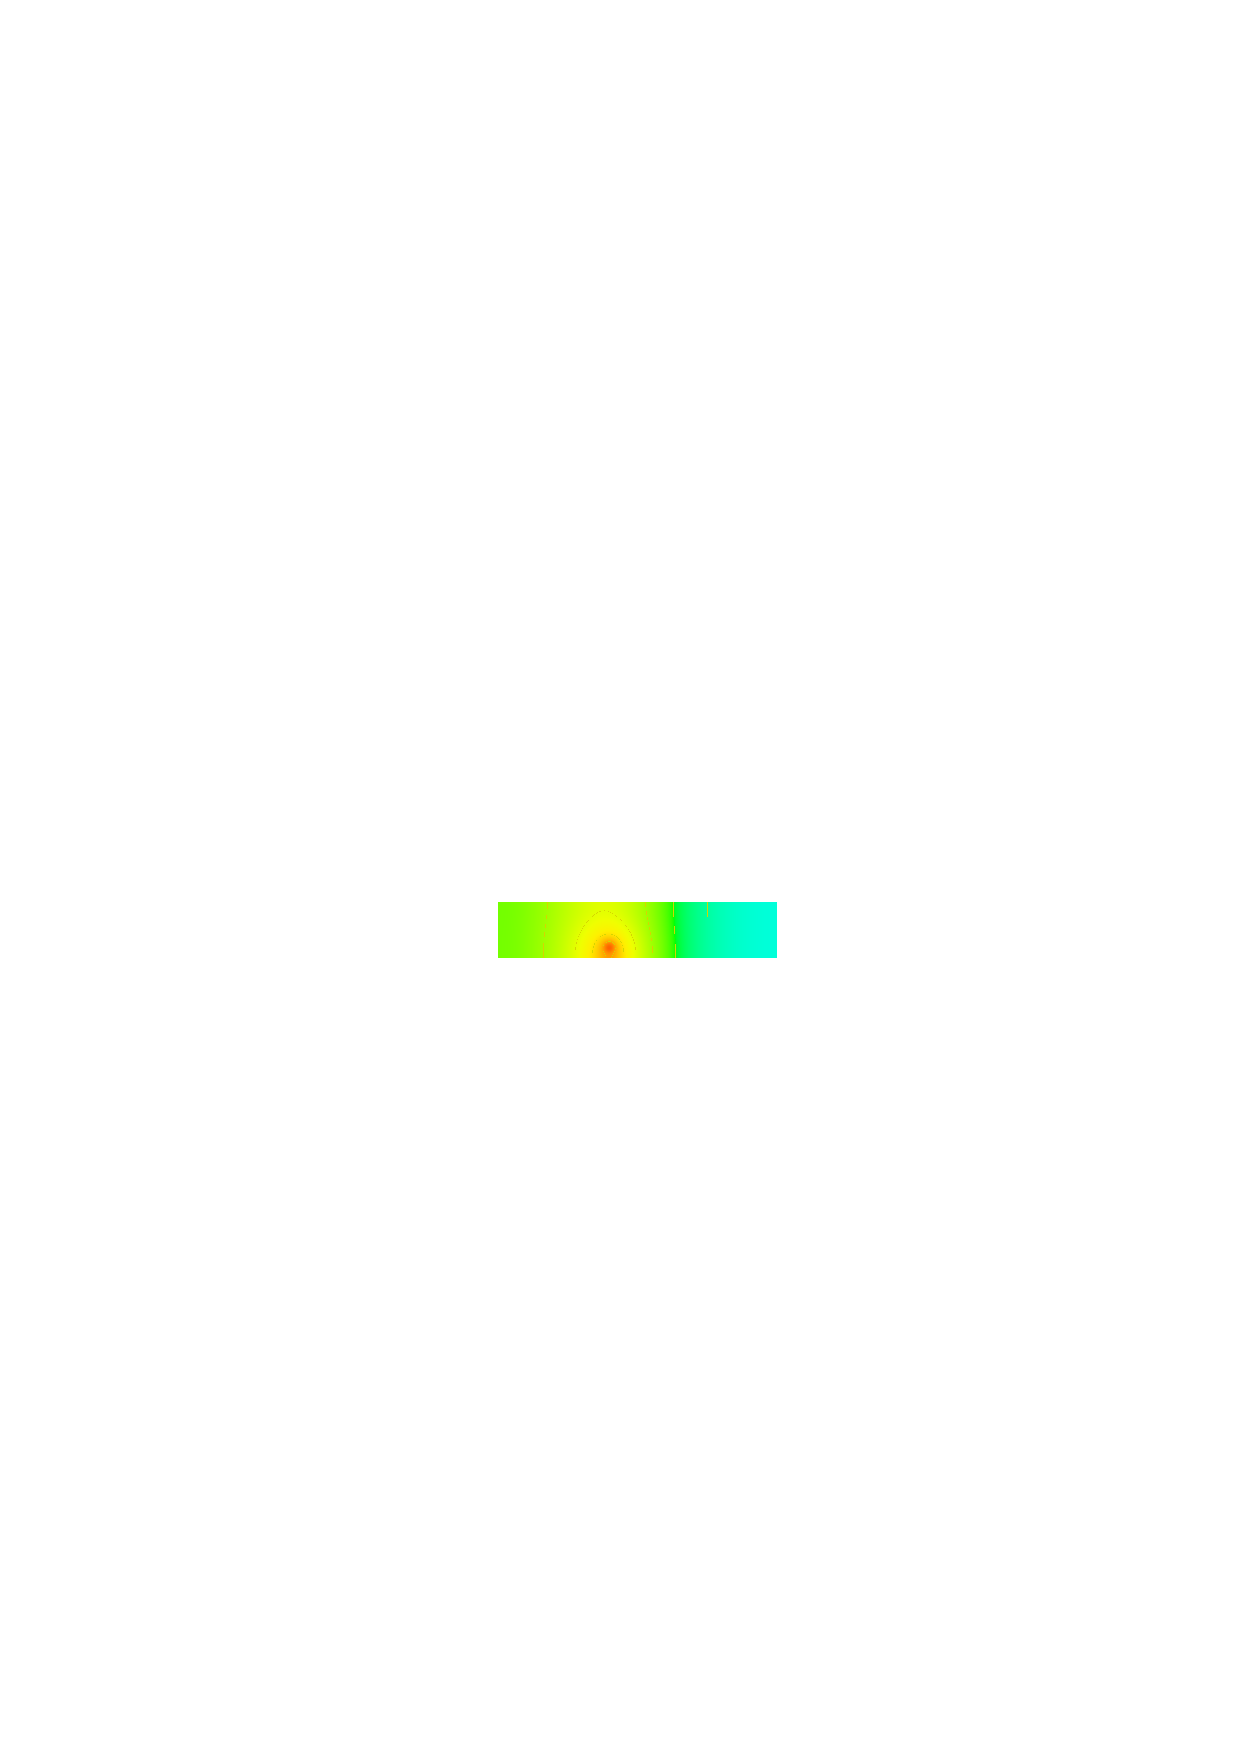
\includegraphics[width=\figwidth]{DiffusionRes48}}
\caption{Results of the Temperture Diffusion Problem for Time Steps $1$ $16$, $32$ and $48$.}
\label{DIFFUSION FIG 2}
\end{figure}

An easy way to visualize the results is the command
\begin{verbatim}
dx -edit diffusion.net &
\end{verbatim}
where \file{diffusion.net} is an \OpenDX script available in the \ExampleDirectory.
Use the \texttt{Sequencer} to move forward and and backwards in time. 
\fig{DIFFUSION FIG 2} shows the result for some selected time steps.
